%%%%%%%%%%%%%%%%%%%%%%%%%%%%%%%%%%%%%%%%%
% Beamer Presentation
% LaTeX Template
% Version 1.0 (10/11/12)
%
%
% License:
% CC BY-NC-SA 3.0 (http://creativecommons.org/licenses/by-nc-sa/3.0/)
%
%%%%%%%%%%%%%%%%%%%%%%%%%%%%%%%%%%%%%%%%%

%----------------------------------------------------------------------------------------
%	PACKAGES AND THEMES
%----------------------------------------------------------------------------------------

\documentclass{beamer}


\documentclass{article}
\usepackage[english]{babel}
\usepackage[utf8x]{inputenc}

\usepackage{CJKutf8}
\usepackage{expex}
\usepackage{enumerate}

\usepackage{apacite}



\usepackage{apacite}

\mode<presentation> {

% The Beamer class comes with a number of default slide themes
% which change the colors and layouts of slides. Below this is a list
% of all the themes, uncomment each in turn to see what they look like.

%\usetheme{default}
\usetheme{AnnArbor}
%\usetheme{Antibes}
%\usetheme{Bergen}
%\usetheme{Berkeley}
%\usetheme{Berlin}
%\usetheme{Boadilla}
%\usetheme{CambridgeUS}
%\usetheme{Copenhagen}
%\usetheme{Darmstadt}
%\usetheme{Dresden}
%\usetheme{Frankfurt}
%\usetheme{Goettingen}
%\usetheme{Hannover}
%\usetheme{Ilmenau}
%\usetheme{JuanLesPins}
%\usetheme{Luebeck}
%\usetheme{Madrid}
%\usetheme{Malmoe}
%\usetheme{Marburg}
%\usetheme{Montpellier}
%\usetheme{PaloAlto}
%\usetheme{Pittsburgh}
%\usetheme{Rochester}
%\usetheme{Singapore}
%\usetheme{Szeged}
%\usetheme{Warsaw}

% As well as themes, the Beamer class has a number of color themes
% for any slide theme. Uncomment each of these in turn to see how it
% changes the colors of your current slide theme.

%\usecolortheme{albatross}
\usecolortheme{beaver}
%\usecolortheme{beetle}
%\usecolortheme{crane}
%\usecolortheme{dolphin}
%\usecolortheme{dove}
%\usecolortheme{fly}
%\usecolortheme{lily}
%\usecolortheme{orchid}
%\usecolortheme{rose}
%\usecolortheme{seagull}
%\usecolortheme{seahorse}
%\usecolortheme{whale}
\usecolortheme{wolverine}
\setbeamercovered{transparent}
%\setbeamertemplate{footline} % To remove the footer line in all slides uncomment this line
\setbeamertemplate{footline}[page number] % To replace the footer line in all slides with a simple slide count uncomment this line

%\setbeamertemplate{navigation symbols}{} % To remove the navigation symbols from the bottom of all slides uncomment this line
}

\usepackage{graphicx} % Allows including images
\usepackage{booktabs} % Allows the use of \toprule, \midrule and \bottomrule in tables

%----------------------------------------------------------------------------------------
%	TITLE PAGE
%----------------------------------------------------------------------------------------

\title[Short title]{The primacy of animacy for the subject grammatical function in Mandarin Chinese} % The short title appears at the bottom of every slide, the full title is only on the title page

\author{Shaohua Fang \& Alan Juffs} % Your name
\institute[PITT] % Your institution as it will appear on the bottom of every slide, may be shorthand to save space
{
University of Pittsburgh \\ % Your institution for the title page
\medskip
\textit{shf64@pitt.edu} % Your email address
}
\date{\today} % Date, can be changed to a custom date

\begin{document}

\begin{frame}
\titlepage % Print the title page as the first slide
\end{frame}


%----------------------------------------------------------------------------------------
%	PRESENTATION SLIDES
%----------------------------------------------------------------------------------------


%------------------------------------------------

\begin{frame}
\frametitle{Sentence comprehension \& event structure representation}

\begin{enumerate}
    \pause
    \item Sentence comprehension involves the rapid integration of different types of linguistic cues.
    \pause
   \setlength{\parskip}{1em}
   \pause
   \item Different cues compete for sentence interpretation (MacWhinney, 2008)
 
   \pause
   \begin{itemize}
   \pause
     \item Different cues weighted differently crosslinguistically (Harrington, 1987).
     \pause
     \begin{itemize}
     \pause
        \item Word order - English ; animacy- Japanese
        \pause
     \end{itemize}
   \end{itemize}
   %\setlength{\parskip}{1em}
   \pause
   \item Linguistic cues used to build up event representation during sentence comprehension \Rightarrow \text{“who did what to whom”}
   
    \pause
    \begin{itemize}
    \pause
        \item English reversible passives cause misinterpretation and processing difficulty (Stromswold et al., 2002; Ferreira, 2003)
            \pause
            \begin{itemize}
            \pause
            \item e.g., The coyote was chased by the dog.
            \pause
            \end{itemize}
   \end{itemize}
\end{enumerate}

\end{frame}

%------------------------------------------------


%------------------------------------------------

\begin{frame}
\frametitle{Linguistic facts about Chinese}

\begin{enumerate}
    \pause
   \item Relatively flexible word order - SVO, SOV etc.
   \pause
   \setlength{\parskip}{1em}
   \pause
   \item No rich inflectional morphemes
   \pause
   \begin{itemize}
    \pause
       \item \emph{ba} \& \emph{bei} as free morphemes used to signal grammatical relation
       \vspace{2mm}
       \begin{CJK*}{UTF8}{gbsn}itemize
       
       \begin{itemize}
           \centering
           \item[(1)] 小男孩把小女孩叫醒了。
           \vspace{1mm}
           \item[(2)] 小男孩被小女孩叫醒了。
       \end{itemize}
    
       %\begin{exe}
       %\ex 小男孩把小女孩叫醒了。
       %\ex 小男孩被小女孩叫醒了。
       %\end{exe}
       
       \end{CJK*}
       \pause
   \end{itemize}
   \setlength{\parskip}{1em}
   \pause
   \item Animacy as a semantic feature of arguments
   \pause
    \begin{itemize}
    \pause
    \item Prototypical semantic role for animate NPs as agent
    \pause
   \end{itemize}
\end{enumerate}
\end{frame}

%------------------------------------------------



%------------------------------------------------

\begin{frame}
\frametitle{Experimental evidence}
\begin{enumerate}
   \item Li, Bates & MacWhinney (1993)
   \setlength{\parskip}{1em}
   \begin{itemize}
       \item bei $> $animacy$> $word order$>$ ba
   \end{itemize}
   \setlength{\parskip}{1em}
   \item Philipp et al. (2008)
    \begin{itemize}
    \item No animacy effect for NP1 but for NP2
   \end{itemize}
   \item Feng et al. (2015)
   \setlength{\parskip}{1em}
   \begin{itemize}
       \item animacy$ > $word order
   \end{itemize}
   \setlength{\parskip}{1em}
   \item Huang et al. (2013) & Zhou \& Ma(2018)
    \begin{itemize}
    \item bei=ba, animacy controlled
   \end{itemize}
\end{enumerate}
\frametitle{Experimental evidence}
\centering
\pause
\textbf{\textcolor{blue}{Divergent results}}
\pause
\end{frame}

%------------------------------------------------



%------------------------------------------------

\begin{frame}
\frametitle{The present study}
\begin{block}{Generally:}
\begin{itemize}
    \pause
    \item We examine the effects of morphosyntactic markers (ba/bei), NP animacy and word order on the off-line processing of ba- and bei-construction by Chinese native speakers.
    \pause
\end{itemize}
\end{block}

\begin{block}{Specifically:}
\begin{itemize}
    \pause
    \item Investigate the interaction among linguistic cues during sentence comprehension (Exp1)
    \pause
    \pause
    \item Adverbials added to create discourse context for the baseline of SPR and Eye-tracking experiments (Exp2)
    \pause
\end{itemize}
\end{block}

\end{frame}

%------------------------------------------------



%------------------------------------------------
\begin{frame}
\frametitle{Experiment 1: AJ Paradigm}
\begin{enumerate}
    \pause
    \item Acceptability judgment (N=149, 64 items)
    \pause
    \begin{itemize}
        \pause
        \item 7-point Likert Scale (both ends labeled)
        \item 1-7 (1=completely unacceptable; 7=completely acceptable)
        \pause
    \end{itemize}
\end{enumerate}
\end{frame}

%------------------------------------------------


%------------------------------------------------
\begin{frame}
\frametitle{Experimental design}
\begin{enumerate}
    \pause
    \item 2*2*2 factorial design
    \pause
    \begin{itemize}
        \pause  
        \item NP1 was manipulated as Animate or Inanimate
        \item NP2 was Animate  or Inanimate
        \item Marker as \emph{ba} or \emph{bei}
        \pause
    \end{itemize}
\end{enumerate}
\end{frame}

%------------------------------------------------


%------------------------------------------------
\begin{frame}
\frametitle{Data processing}
\begin{enumerate}
    \item Z-score transformation to mitigate scale bias and unequal intervals
        \textbf\centering{\textcolor{blue}{\[ z = (\gamma - \mu)/ \sigma \]}}
    \pause
    \item Linear mixed-effects models for statistical analyses 
\end{enumerate}
\end{frame}

%------------------------------------------------


%------------------------------------------------

\begin{frame}
\frametitle{Results}
\begin{columns}[c] % The "c" option specifies centered vertical alignment while the "t" option is used for top vertical alignment

\column{0.7\textwidth} % Left column and width
\begin{figure}
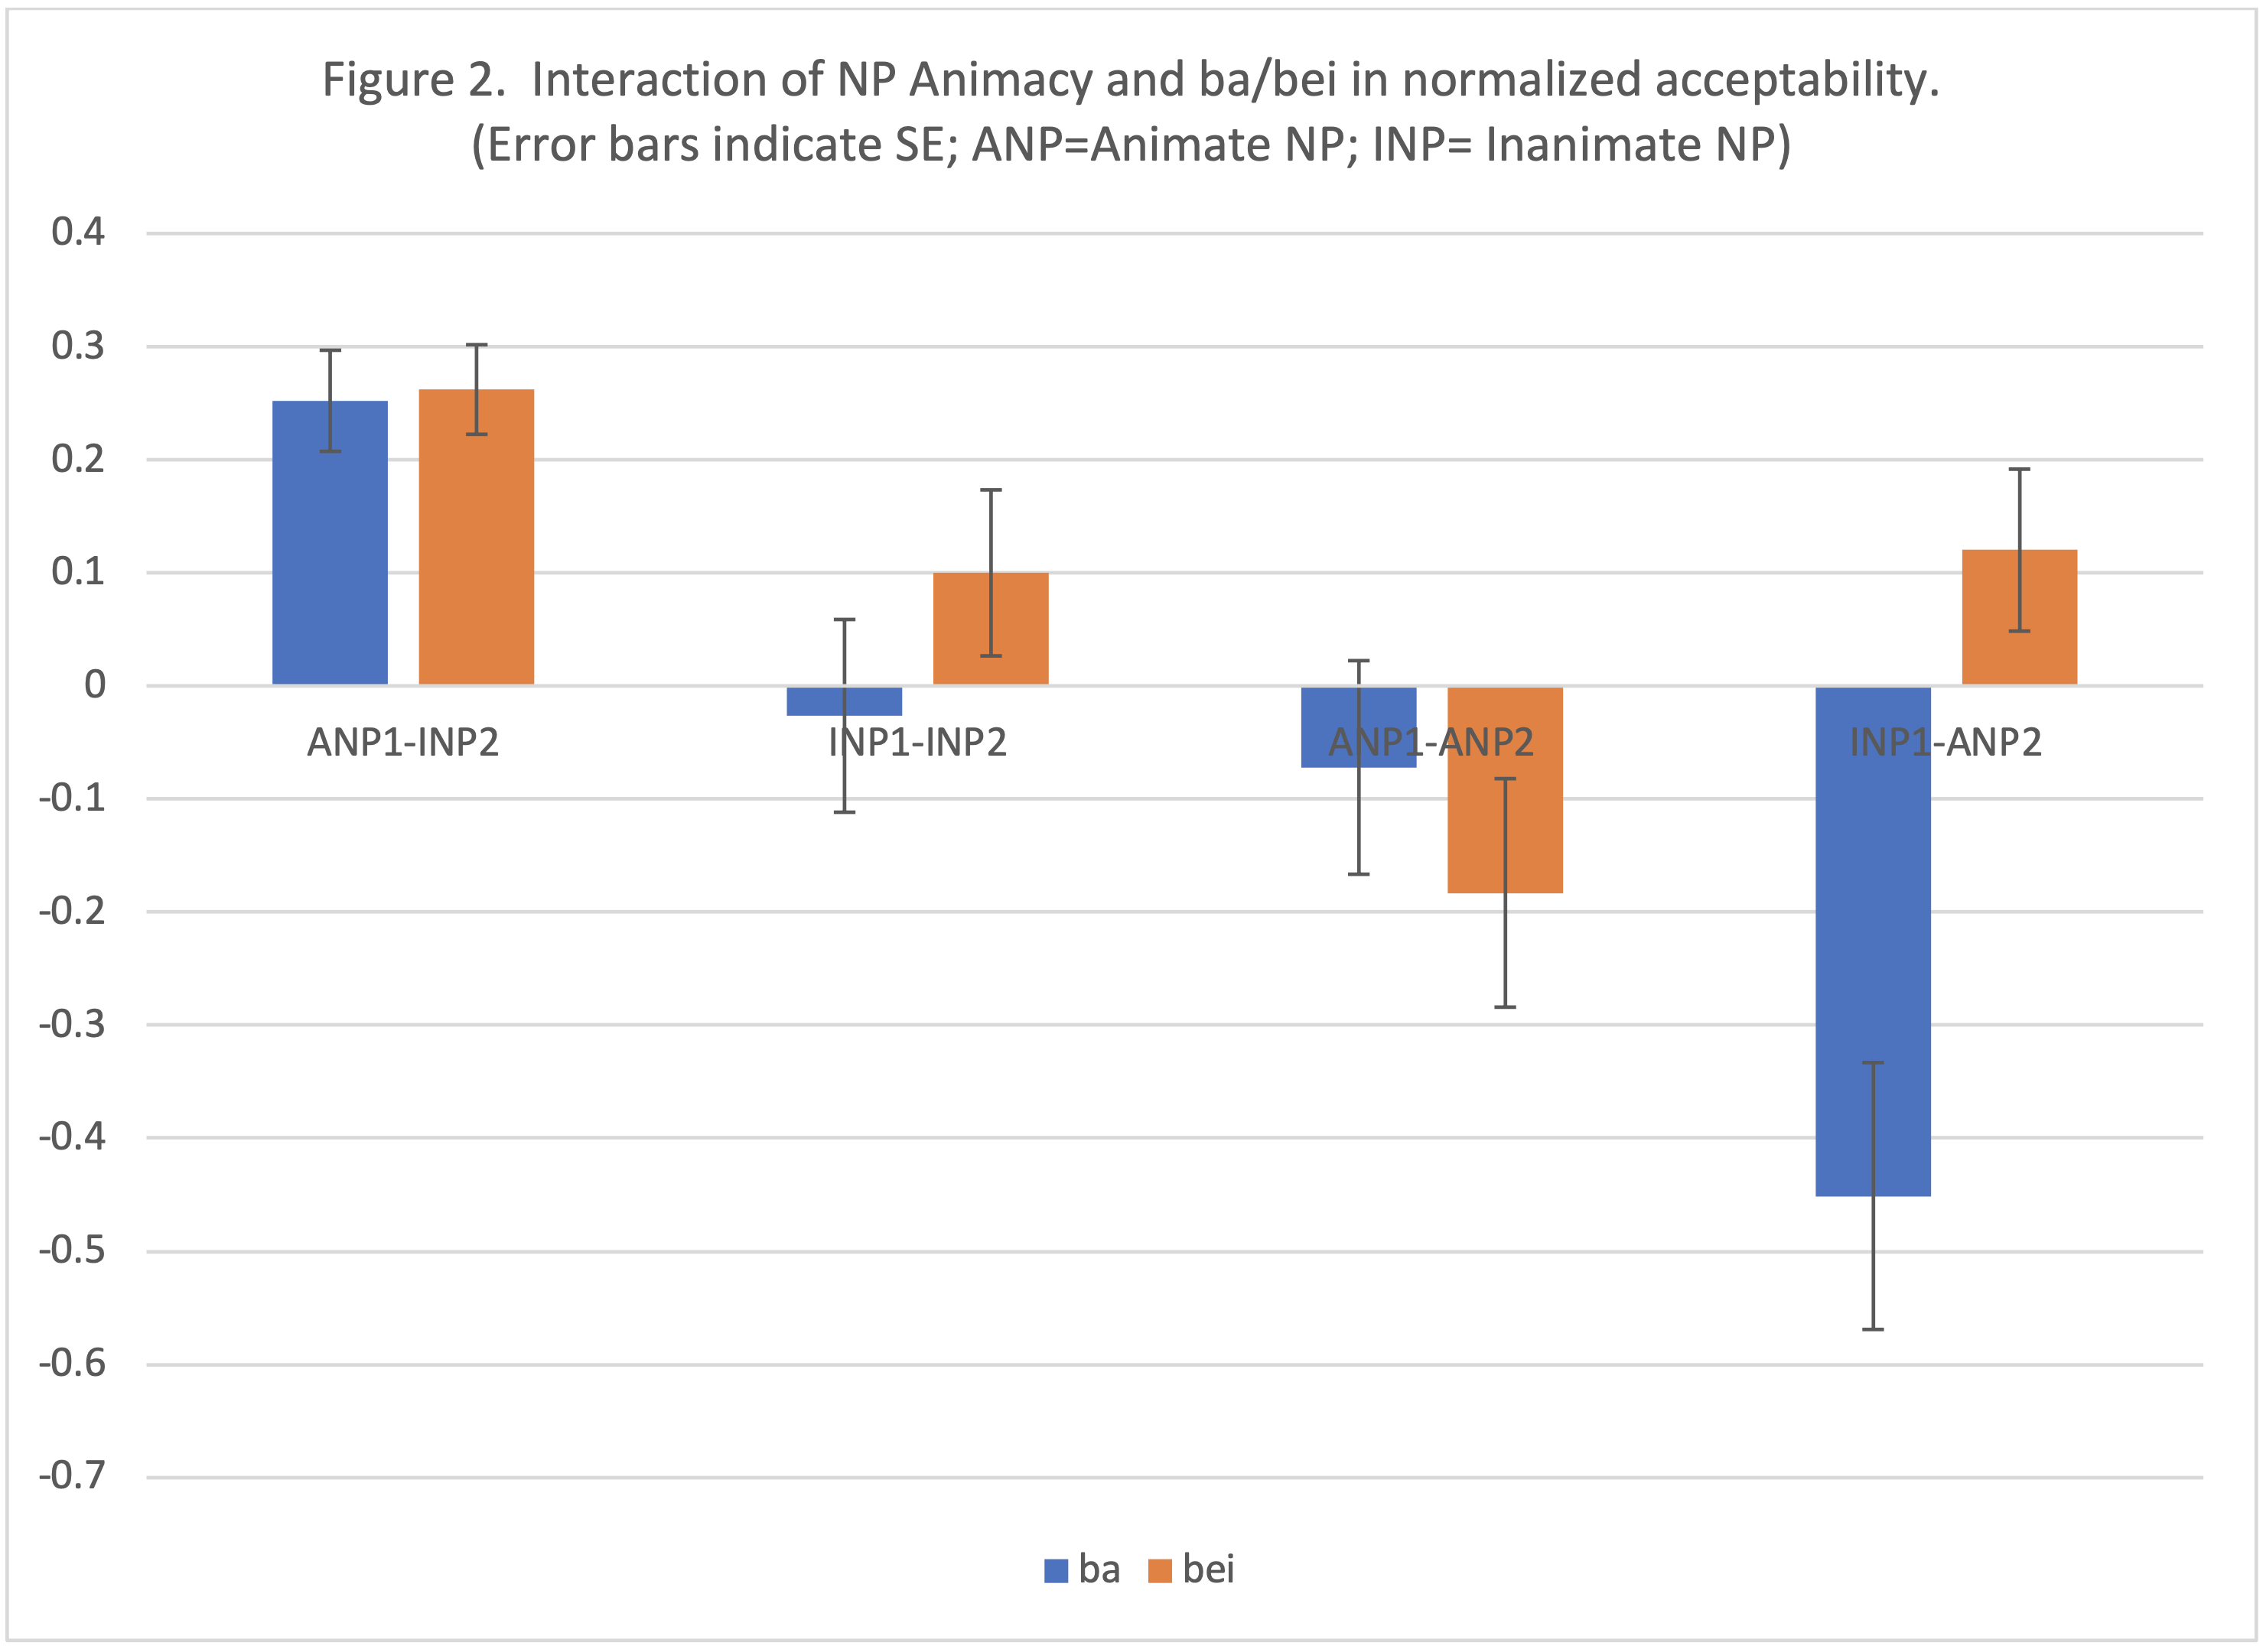
\includegraphics[width=8cm,height=7cm,keepaspectratio]{SHF_Presentation/Exp1.png}
\end{figure}

\column{.3\textwidth} % Right column and width

{\scriptsize
\begin{itemize}
    \item<1-> Constructions with animate NP1 preferred
    \item<2-> Constructions with inanimate NP2 preferred 
    \item<3-> Bei-constructions preferred
    \item<4-> NP1 and NP2 tend to be contrastive in animacy 
    \item<5-> Ba-constructions prefer animate NP1s and Bei-constructions prefer inanimate NP1 when NP2s are animate
\end{itemize}
}
\end{columns}
\end{frame}

%------------------------------------------------

\begin{frame}
\frametitle{Takeaway}

\begin{enumerate}
    \pause
    \item Animacy effect for NP1 and NP2.
    \pause
   \setlength{\parskip}{1em}
   \pause
   \item Animacy and morphosyntactic cues interact for interpretation 
   \pause
   \item Animacy contrast facilitates the activation of animacy cues during processing (Ferreira, 2003) 
\end{enumerate}
\end{frame}

%------------------------------------------------

\begin{frame}
\frametitle{Experiment 2}

\begin{enumerate}
    \item Paradigm 
    \begin{itemize}
        \item Naturalness judgment test (N=112, 64 items)
    \end{itemize}
   \item Design: 2*2*2
   \item Material 
   \begin{itemize}
       \item NP modifier and adverbs added to prepare for online experiments
   \end{itemize}
\begin{figure}
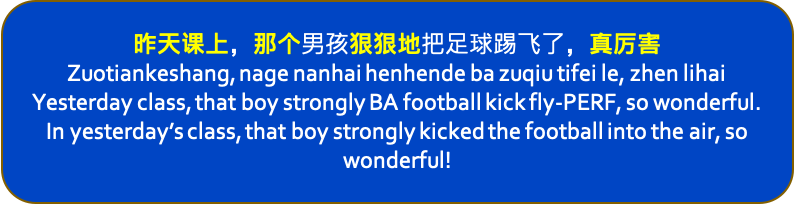
\includegraphics[width=8cm,height=6cm,keepaspectratio]{SHF_Presentation/Example.png}
\end{figure}
\end{enumerate}
\end{frame}

%------------------------------------------------


%------------------------------------------------

\begin{frame}
\frametitle{Results}
\begin{columns}[c] % The "c" option specifies centered vertical alignment while the "t" option is used for top vertical alignment

\column{0.7\textwidth} % Left column and width
\begin{figure}
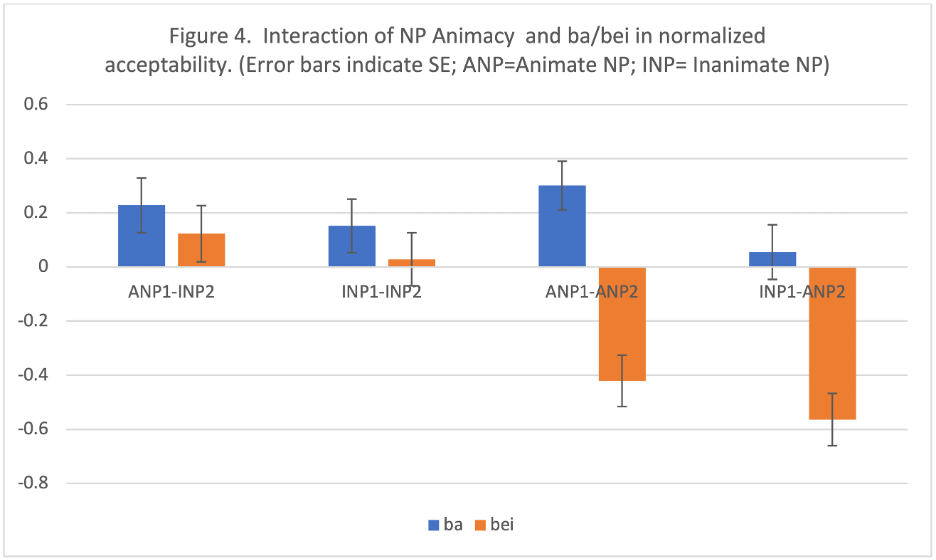
\includegraphics[width=8cm,height=7cm,keepaspectratio]{SHF_Presentation/Exp2.png}
\end{figure}

\column{.3\textwidth} % Right column and width

{\footnotesize
\begin{itemize}
    \item<1-> Constructions with animate NP1 preferred
    \item<2-> Constructions with inanimate NP2 preferred 
    \item<3-> Ba-constructions preferred
    \item<4-> Regardless of the animacy of NP1, bei-constructions strongly favor inanimate NP2
\end{itemize}
}

\end{columns}
\end{frame}

%------------------------------------------------



%------------------------------------------------

\begin{frame}
\frametitle{Takeaway}
\begin{enumerate}
   \item Animacy effect for NP1 and NP2
   \setlength{\parskip}{1em}
   \item Regardless of the animacy of NP1, bei-constructions strongly favor inanimate NP2, which may suggest a shallow processing strategy (Ferreira, Bailey & Ferraro, 2002) \Rightarrow \text{NP1-NP2: agent – theme} 
   
\begin{figure}
\pause
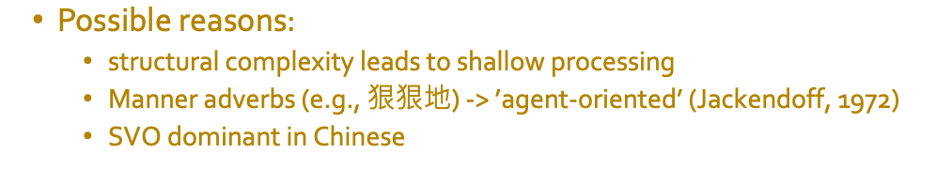
\includegraphics[width=10cm,height=10cm,keepaspectratio]{SHF_Presentation/PossibleReason.png}
\pause
\end{figure} 

\end{enumerate}
\end{frame}

%------------------------------------------------

%------------------------------------------------

\begin{frame}
\frametitle{Conclusions \& implications}

\begin{enumerate}
    \pause
   \item Animacy serves as a primary cue but also interacts with other cues to determine interpretation in Chinese
   \pause
   \setlength{\parskip}{1em}
   \pause
   \item Online measures to identify location of processing difficulty 
   \pause
   \item The effect of adverbs to be controlled
   \pause
   \item These factors are important for interlanguage development and processing 
\end{enumerate}
\end{frame}

%------------------------------------------------
\begin{frame}[shrink=15]
\frametitle{Selected references}

\nocite{*}   % this is to print out bibliography without including in-text citation
\bibliographystyle{apacite}
\bibliography{references}

\end{frame}


%------------------------------------------------

\begin{frame}
\Huge{\centerline{Thank you!}}
\begin{CJK*}{UTF8}{bsmi}
\Huge{\centerline{謝謝!}}
\end{CJK*}
\vspace{10mm}
\noindent\rule{\textwidth}{1pt}
\fontsize{10pt}{12pt}\selectfont
\begin{center}
    We thank Yi Xu, Melinda Frick, Jon Sprouse, Wuyue Liang and Hui Zhang for their help with this project.
\end{center}
    
%\setlength{\parskip}{1em}
%\text{\normalsize We thank Yi Xu, Melinda Frick, Jon Sprouse, Wuyue Liang and Hui Zhang for their help with this project}
\end{frame}

%----------------------------------------------------------------------------------------

\end{document} 